\documentclass[unknownkeysallowed]{beamer}
\usepackage[french,english]{babel}

\usepackage{pythontex}
\usepackage[english]{babel}
\usepackage{xcolor}
\usepackage{movie15}
\usepackage{amssymb}
\usepackage{amsthm}
\usepackage{amsfonts}
\usepackage[utf8]{inputenc}
\usepackage{pythontex}
\usepackage{fontawesome}
\usetheme{Madrid}
% \DeclareMathOperator*{\argmin}{arg\,min}
% \usecolortheme{beaver}
% \usetheme{Boadilla}
\usepackage{utopia}%font utopia imported
\usepackage{graphicx}
\newtheorem{exmp}{Exemple}[section]
\usepackage{amsmath}
\usepackage{stmaryrd}
\usecolortheme{beaver}
\renewcommand{\contentsname}{Table des matières}
\usepackage{../../../sty/beamer_js} % Missing package, see  https://github.com/josephsalmon/OrganizationFiles/tree/master/tex/sty
\usepackage{../../../sty/shortcuts_js} % Missing package, see  https://github.com/josephsalmon/OrganizationFiles/tree/master/tex/sty

\begin{document}


%%%%%%%%%%%%%%%%%%%%%%%%%%%%%%%%%%%%%%%%%%%%%%%%%%%%%%%%%%%%%%%%%%%%%%%%%%%%%%%
%%%%%%%%%%%%%%%%%%%%%%             Headers               %%%%%%%%%%%%%%%%%%%%%%
%%%%%%%%%%%%%%%%%%%%%%%%%%%%%%%%%%%%%%%%%%%%%%%%%%%%%%%%%%%%%%%%%%%%%%%%%%%%%%%



%%%%%%%%%%%%%%%%%%%%%%%%%%%%%%%%%%%%%%%%%%%%%%%%%%%%%%%%%%%%%%%%%%%%%%%%%%%%%%%
\begin{frame}
\bigskip
\bigskip
\begin{center}{
\LARGE\color{marron}
\textbf{HMMA 307 : Advanced Linear Modeling}
\textbf{ }\\
\vspace{0.5cm}
}

\color{marron}
\textbf{Chapter 2 : Optimization under constraints}
\end{center}

\vspace{0.25cm}

\begin{center}
\textbf{Delage Cindy, \ Hanna Bacave \ and \ Ruoyu Wang \\}
\faGithub\href{ https://github.com/hannabacave/MLA}{ Linear Model Advanced}
\\
\vspace{0.5cm}
Université de Montpellier \\
\end{center}

\centering

\includegraphics[width=0.13\textwidth]{umonpellier_logo}

\end{frame}
%%%%%%%%%%%%%%%%%%%%%%%%%%%%%%%%%%%%%%%%%%%%%%%%%%%%%%%%%%%%%%%%%%%%%%%%%%%%%%%



%%%%%%%%%%%%%%%%%%%%%%%%%%%%%%%%%%%%%%%%%%%%%%%%%%%%%%%%%%%%%%%%%%%%%%%%%%%%%%%
%%%%%%%%%%%%%%%%%%%%%%%%       PLAN      %%%%%%%%%%%%%%%%%%%%%%%%%%%%%%%%%%%%%%
%%%%%%%%%%%%%%%%%%%%%%%%%%%%%%%%%%%%%%%%%%%%%%%%%%%%%%%%%%%%%%%%%%%%%%%%%%%%%%%



%%%%%%%%%%%%%%%%%%%%%%%%%%%%%%%%%%%%%%%%%%%%%%%%%%%%%%%%%%%%%%%%%%%%%%%%%%%%%%%
\begin{frame}{Table of Contents}
\tableofcontents[hideallsubsections]
\end{frame}
%%%%%%%%%%%%%%%%%%%%%%%%%%%%%%%%%%%%%%%%%%%%%%%%%%%%%%%%%%%%%%%%%%%%%%%%%%%%%%%



%%%%%%%%%%%%%%%%%%%%%%%%%%%%%%%%%%%%%%%%%%%%%%%%%%%%%%%%%%%%%%%%%%%%%%%%%%%%%%%
\AtBeginSection[]
{
\begin{frame}<beamer>{Table of Contents}
\tableofcontents[currentsubsection,
    hideothersubsections,
    sectionstyle=show/shaded,
]
\end{frame}
}
%%%%%%%%%%%%%%%%%%%%%%%%%%%%%%%%%%%%%%%%%%%%%%%%%%%%%%%%%%%%%%%%%%%%%%%%%%%%%%%




%%%%%%%%%%%%%%%%%%%%%%%%%%%%%%%%%%%%%%%%%%%%%%%%%%%%%%%%%%%%%%%%%%%%%%%%%%%%%%%
%%%%%%%%%%%%%%%%%%%%%%%%%%%%%%%%%%%%%%%%%%%%%%%%%%%%%%%%%%%%%%%%%%%%%%%%%%%%%%%
\section{Convexity reminder}
\label{sec:Convexity reminder}
%%%%%%%%%%%%%%%%%%%%%%%%%%%%%%%%%%%%%%%%%%%%%%%%%%%%%%%%%%%%%%%%%%%%%%%%%%%%%%
%%%%%%%%%%%%%%%%%%%%%%%%%%%%%%%%%%%%%%%%%%%%%%%%%%%%%%%%%%%%%%%%%%%%%%%%%%%%%%%
%%%%%%%%%%%%%%%%%%%%%%%%%%%%%%%%%%%%%%%%%%%%%%%%%%%%%%%%%%%%%%%%%%%%%%%%%%%%%%%


%%%%%%%%%%%%%%%%%%%%%%%%%%%%%%%%%%%%%%%%%%%%%%%%%%%%%%%%%%%%%%%%%%%%%%%%%%%%%%%
\begin{frame}{Convexity reminder}
\begin{alertblock}{Theorem}
Consider a function $f :
\begin{array}{l rcl}
 & \mathbb{R}^d & \longrightarrow & \mathbb{R}^d \\
    & x & \longmapsto & f(x)
\end{array}$, if $f$ is convex and $\mathcal{C}^1$, then
    $$x^{\star} \in \argmin_{x \in \mathbb{R}^d } f(x) \Leftrightarrow \nabla f(x^{\star}) = 0$$
\end{alertblock}
\vspace{0.4cm}
\begin{block}{Remark}
f convex and $\mathcal{C}^1 \Leftrightarrow \forall x_1 \in \mathbb{R}^d, \forall x_2 \in \mathbb{R}^d$,
 $$f(x) \geq f(x_1) \   + <\nabla f(x_1), x_1-x_2>$$
\end{block}
\end{frame}


%%%%%%%%%%%%%%%%%%%%%%%%%%%%%%%%%%%%%%%%%%%%%%%%%%%%%%%%%%%%%%%%%%%%%%%%%%%%%%%

%%%%%%%%%%%%%%%%%%%%%%%%%%%%%%%%%%%%%%%%%%%%%%%%%%%
%%%%%%%%%%%%%%%%%%%%%%%%%%%%%%%%%%%%%%%%%%%%%%%%%%%%%%%%%%%%%%%%%%%%%%%%%%%%%%%



%%%%%%%%%%%%%%%%%%%%%%%%%%%%%%%%%%%%%%%%%%%%%%%%%%%%%%%%%%%%%%%%%%%%%%%%%%%%%%%

%%%%%%%%%%%%%%%%%%%%%%%%%%%%%%%%%%%%%%%%%%%%%%%%%%%%%%%%%%%%%%%%%%%%%%%%%%%%%%%
%%%%%%%%%%%%%%%%%%%%%%%%%%%%%%%%%%%%%%%%%%%%%%%%%%%%%%%%%%%%%%%%%%%%%%%%%%%%%%%
\section{Optimization under constraints}
\label{sec:conclusion}
%%%%%%%%%%%%%%%%%%%%%%%%%%%%%%%%%%%%%%%%%%%%%%%%%%%%%%%%%%%%%%%%%%%%%%%%%%%%%%%
%%%%%%%%%%%%%%%%%%%%%%%%%%%%%%%%%%%%%%%%%%%%%%%%%%%%%%%%%%%%%%%%%%%%%%%%%%%%%%%
\begin{frame}
\frametitle{Model implementation}
\begin{block}{Target}
The target is to reach optimum of the function $f_0 : \begin{array}{l rcl}
 & \mathbb{R}^d & \longrightarrow & \mathbb{R}^d \\
    & x & \longmapsto & f_0(x)
\end{array}$ under constraints.
\end{block}
\vspace{0.5cm}
We apply $n_1$ inegality constraints and $n_2$ egality constraints at $f_0$, like :
\begin{itemize}
    \item $f_i(x)\  \leq \  0 \  \ \forall i \in \{1, \cdots , n_1\}$ ;
    \item $h_j(x)\  = \  0 \  \ \forall j \in \{1, \cdots , n_2\}$ .
\end{itemize}
\vspace{0.25cm}
To achieve the goal, we need to suppose that :
\begin{itemize}
    \item $f_0$ and $\forall i, \forall j, \ f_i$, $h_j$ are $\mathcal{C}^1$ ;
    \item $f_0$ and $\forall i ,  f_i$ are convex.
\end{itemize}
\end{frame}

%%%%%%%%%%%%%%%%%%%%%%%%%%%%%%%%%%%%%%%%%%%%%%%%%%%%%%%%%%%%%%%%%%%%%%%%%%%%%%%
\begin{frame}
\frametitle{Model implementation}
\begin{block}{Definition}
We define the \textit{feasability set} as $\mathcal{F} = \{x \in \mathbb{R}^d \ / \  \forall i=1,...,n_1, f_i(x)\leq 0 $ and $\forall j=1,...,n_2, \ h_j(x)=0\}$
\end{block}
\vspace{0.3cm}
We get the following problem :
\begin{alertblock}{Constrained problem}
$$\min_{x \in \mathcal{F}} f_0\,(x)$$
\end{alertblock}
\vspace{0.3cm}
\begin{block}{Definition}
We define the \textit{primal value} (\textit{optimal value}) of constrained problem by $$p^{\star} = \min_{x \in \mathcal{F}} f_0\,(x)$$
\end{block}
\end{frame}

%%%%%%%%%%%%%%%%%%%%%%%%%%%%%%%%%%%%%%%%%%%%%%%%%%%%%%%%%%%%%%%%%%%%%%%%%%%%%%%

\begin{frame}
\begin{block}{Definition}
We call \textit{Lagrangian} (or \textit{Lagrangian multiplier}) the function such that $\forall \, x \in \mathbb{R}^d, \lambda \in \mathbb{R}^{n_{1}}$ and $\nu \in \mathbb{R}^{n_{2}}$:
$$\mathcal{L}(x,\lambda,\nu) = f_0\,(x) + \sum_{i=1}^{n_1} \lambda_i \, f_i\,(x) + \sum_{j=1}^{n_2} \nu_j \, h_j\,(x) $$
\end{block}
\end{frame}

%%%%%%%%%%%%%%%%%%%%%%%%%%%%%%%%%%%%%%%%%%%%%%%%%%%%%%%%%%%%%%%%%%%%%%%%%%%%%%%

\begin{frame}
\begin{block}{Definition}
\begin{center}
$g & : & \mathbb{R}^{n_{1}} * \mathbb{R}^{n_{2}} & \to & \mathbb{R} \\
 & & (\lambda,\nu) & \mapsto & \displaystyle \min_{x \in \mathbb{R}^d} \, \mathcal{L}(x,\lambda,\nu) \\$
 \end{center}
 is the \textit{dual function} of the problem.
\end{block}
\begin{block}{Comments}
\begin{itemize}
\item g is a concave function (minimum of affine functions)
\item \forall $\lambda \geq 0 \, (\lambda_1 \geq 0, ..., \lambda_{n_{1}}\geq0)$  and  $\forall \, x \in \mathcal{F}$ we have :
\begin{align*}
 \mathcal{L}(x,\lambda,\nu) &=  f_0\,(x) + \underbrace{ \sum_{i=1}^{n_1} \lambda_i \, f_i\,(x)} _{\leq \, 0} + \underbrace{ \sum_{j=1}^{n_2} \nu_j \, h_j\,(x) }_{= \, 0} \\ &\leq f_0\,(x).
\end{align*}
\end{itemize}
\end{block}
\end{frame}

 %%%%%%%%%%%%%%%%%%%%%%%%%%%%%%%%%%%%%%%%%%%%%%%%%%%%%%%%%%%%%%%%%%%%%%%%%%%%%%

 \begin{frame}
\begin{block}{}
So we have :
\begin{align*}
\forall
\{ \min_{x \in \mathbb{R}^d} \, \mathcal{L}(x,\lambda,\nu )\}_{g(\lambda,\nu)} & \leq f_0(x) \\
g(\lambda,\nu) & \leq \min_{x \in \mathcal{F}} f_0\,(x) = p^{*}.
\end{align*}
\end{block}
\begin{block}{Dual problem}
The \textit{dual problem} consists to find $d^{*} =\displaystyle  \max_{(\lambda,\nu) \in \mathbb{R}^{n_{1}} * \mathbb{R}^{n_{2}}} \, g(\lambda,\nu)$ such as $\lambda \geq 0$.
\end{block}

\end{frame}
 %%%%%%%%%%%%%%%%%%%%%%%%%%%%%%%%%%%%%%%%%%%%%%%%%%%%%%%%%%%%%%%%%%%%%%%%%%%%%%
\begin{frame}
\begin{figure}[!h]
    \begin{center}
   \caption{\label{étiquette} Primal/Dual}
   \includegraphics[width=10cm]{primaldual}
   \end{center}
    \end{figure}
\end{frame}
%%%%%%%%%%%%%%%%%%%%%%%%%%%%%%%%%%%%%%%%%%%%%%%%%%%%%%%%%%%%%%%%%%%%%%%%%%%%%
\begin{frame}
     \begin{block}{Remark}
        $\forall \lambda \geq 0, \forall x $,
        $$
        g(\lambda, \nu) \overbrace{\leq}^{\text{def. of }d^*} d^* \overbrace{\leq}^{\text{weak duality}} p^* \overbrace{\leq}^{\text{def. of } p^*} f_0(x)
        $$

        We call the \textit{strong duality} when $d^*=p^*$.
     \end{block}

     \begin{alertblock}{Theorem}
        If $\forall i \in \llbracket 1,n_1 \rrbracket, f_i$ are convex; $\forall j \in \llbracket 1,n_2 \rrbracket, h_j$ are affine. If $\exists \tilde x \in \mathbb{R}^d$ such as:
        \begin{align*}
            f_i(\tilde x) &< 0, \forall i \in \llbracket 1,n_1 \rrbracket   \\
            h_j(\tilde x) &= 0, \forall j \in \llbracket 1,n_2 \rrbracket
        \end{align*}
        the strong duality is satisfied and
        $$
        d^* = p^*.
        $$
     \end{alertblock}
\end{frame}

%%%%%%%%%%%%%%%%%%%%%%%%%%%%%%%%%%%%%%%%%%%%%%%%%%%%%%%%%%%%%%%%%%%%%%%%%%%%%
\begin{frame}{Consequence of strong duality}
        If $x^* \in \mathbb{R}^d$ is the solution of primal problem $f_0(x)\in\mathbb{R}^d$ and $(\lambda^*,\nu^*) \in \mathbb{R}_{+}^{n_1} \times \mathbb{R}^{n_2}$ is the solution of dual problem $g(\lambda^*,\nu^*)=d^*$, we will have:
        \begin{align*}
            f(x^*) &= p^* = d^* = g(\lambda^*,\nu^*) \\
                   &= \min_{x\in\mathbb{R}^d} (f_0 (x) + \sum_{i=1}^{n_1} \lambda_i f_i(x) + \sum_{j=1}^{n_2} \nu_j h_j(x)) \\
                   &\leq f_0 (x^*) + \sum_{i=1}^{n_1} \underbrace{\lambda_i^*}_{\geq 0} \underbrace{f_i(x^*)}_{\leq 0} + \underbrace{\sum_{j=1}^{n_2} \nu_j^* h_j(x^*).}_{=0}
        \end{align*}
        We deduce that:
        $$
        \sum_{i=1}^{n_1} \lambda_i^* f_i(x^*) = 0 \Longrightarrow  \underbrace{\forall i, \lambda_i^* f_i(x^*) = 0.}_{\textbf{The complementarity problem}}
        $$
\end{frame}
%%%%%%%%%%%%%%%%%%%%%%%%%%%%%%%%%%%%%%%%%%%%%%%%%%%%%%%%%%%%%%%%%%%%%%%%%%%%%%
\begin{frame}
  So, we obtain:
   \begin{itemize}
        \item If $\lambda^* > 0$, then $f_i(x^*) = 0$. (\textit{constraints saturation})
        \item If $f_i(x^*) < 0$, then $\lambda^* = 0$.
    \end{itemize}

    \vspace{1cm}
    \begin{block}{Remark: \textbf{The first order condition}}
        \begin{gather*}
            \nabla_x \mathcal{L} (x^*, \lambda^*, \nu^*) = 0 \\
            \Longleftrightarrow \\
            \nabla_x f_0 (x^*) + \sum_{i=1}^{n_1} \lambda_i^* \nabla_x f_i(x^*) + \sum_{j=1}^{n_2} \nu_j^* \nabla_x h_j(x^*) = 0.
        \end{gather*}

   \end{block}
\end{frame}
%%%%%%%%%%%%%%%%%%%%%%%%%%%%%%%%%%%%%%%%%%%%%%%%%%%%%%%%%%%%
%%%%%%%%%%%%%%%%%%%%%%%%%%%%%%%%%%%%%%%%%%%%%%%%%%%%%%%%%

\begin{frame}{Example}
     If we have $A\in \mathbb{R}^{n \times p},\ b \in \mathbb{R}^n, C \in \mathbb{R}^{r \times p},d \in \mathbb{R}^r$, we need to resolve the least square problem:
     \begin{gather*}
         \min_{x\in\mathbb{R}^p} \qquad \frac{1}{2} \left\Vert Ax - b \right\Vert^2 \\
         \text{s.t.} \quad Cx-d=0.
     \end{gather*}
    We write the Langragian as:
    \[
    \mathcal{L}(x,\nu) = \frac{1}{2} \left\Vert Ax - b \right\Vert^2 + \nu^\top (Cx-d).
    \]
    We need to solve $\nabla_x \mathcal{L} = 0$:
    \[
    \nabla_x \mathcal{L} = A^\top (Ax-b) + C^\top \nu =0 \Longleftrightarrow A^\top Ax^* = A^\top b - C^\top \nu^*.
    \]
        We obtain a linear system:
        \begin{cases}
            Cx^* = d  \qquad \textit{(feasibility)}\\
            A^\top Ax^*=A^\top b - c^\top \nu^*
        \end{cases}.
 \end{frame}
 %%%%%%%%%%%%%%%%%%%%%%%%%%%%%%%%%%%%%%%%%%%%%%%%%%%%%%%%%%%
\section{Implementations}
\label{sec:}
 %%%%%%%%%%%%%%%%%%%%%%%%%%%%%%%%%%%%%%%%%%%%%%
 \begin{frame}{Optimization of hovercraft trajectory - Presentation}
 We are in command of a hovercraft which must pass through k waypoints at certain times given. Our objective is to hit the waypoints at the prescribed times while minimizing fuel use.
To do this, we need to introduce some notations :
\begin{itemize}
    \item k is the number of waypoints ;
    \item $t = 0, 1, ..., T$ is the discretize time ;
    \item $x_t$ is the hovercraft position at t time ;
    \item $v_t$ is the velocity at the time t ;
    \item $u_t$ is the thrust of hovercraft at the time t ;
    \item $w_i$ is the waypoint.
\end{itemize}
 \end{frame}
 %%%%%%%%%%%%%%%%%%%%%%%%%%%%%%%%%%%%%%%%%%%%%%%%%%%%%%%%%%%%%%%%%
 \begin{frame}{Optimization of hovercraft trajectory - Resolution}
\begin{block}{First Model : hiting the waypoints exactly}
We want to reach
$$\min_{x_t, v_t,u_t} \sum\limits_{t=0}^T \|u_t\|^2,$$
under the constraints :
\begin{itemize}
    \item $\forall t = 0, ..., T$,
    \begin{cases}
    x_{t+1} = x_t + v_t \\
    v_{t+1} = v_t + u_t
    \end{cases} ;
    \item $x_0 = v_0 = 0$ ;
    \item $x_t_i = w_i \ \forall i = 1, ..., k$.
\end{itemize}
\end{block}
 \end{frame}
 %%%%%%%%%%%%%%%%%%%%%%%%%%%%%%%%%%%%%%%%%%%%%%%%%%%%%%%%%%%%%
 \begin{frame}{Optimization of hovercraft trajectory - Resolution}
\begin{block}{Second Model : Passing near waypoints}
We want to reach
$$\min_{x_t, v_t,u_t} \sum\limits_{t=0}^T \|u_t\|^2 + \lambda \sum\limits_{t=0}^T \|x_t_i _ w_i\|^2,$$
under the constraints :
\begin{itemize}
    \item $\forall t = 0, ..., T$,
    \begin{cases}
    x_{t+1} = x_t + v_t \\
    v_{t+1} = v_t + u_t
    \end{cases} ;
    \item $x_0 = v_0 = 0$ ;
    \item $x_t_0 = w_0$.
\end{itemize}
\end{block}
Here $\lambda$ controls the tradeoff between making u small and hitting all the waypoints. \\
 \end{frame}
 %%%%%%%%%%%%%%%%%%%%%%%%%%%%%%%%%%%%%%%%%%%%%%%%%%%
 \begin{frame}{Optimization of hovercraft trajectory - Plot}
\begin{figure}[!h]
     \begin{center}
   \caption{\label{étiquette}Resolution thanks to the First Model (left) and the Second Model (right).}
   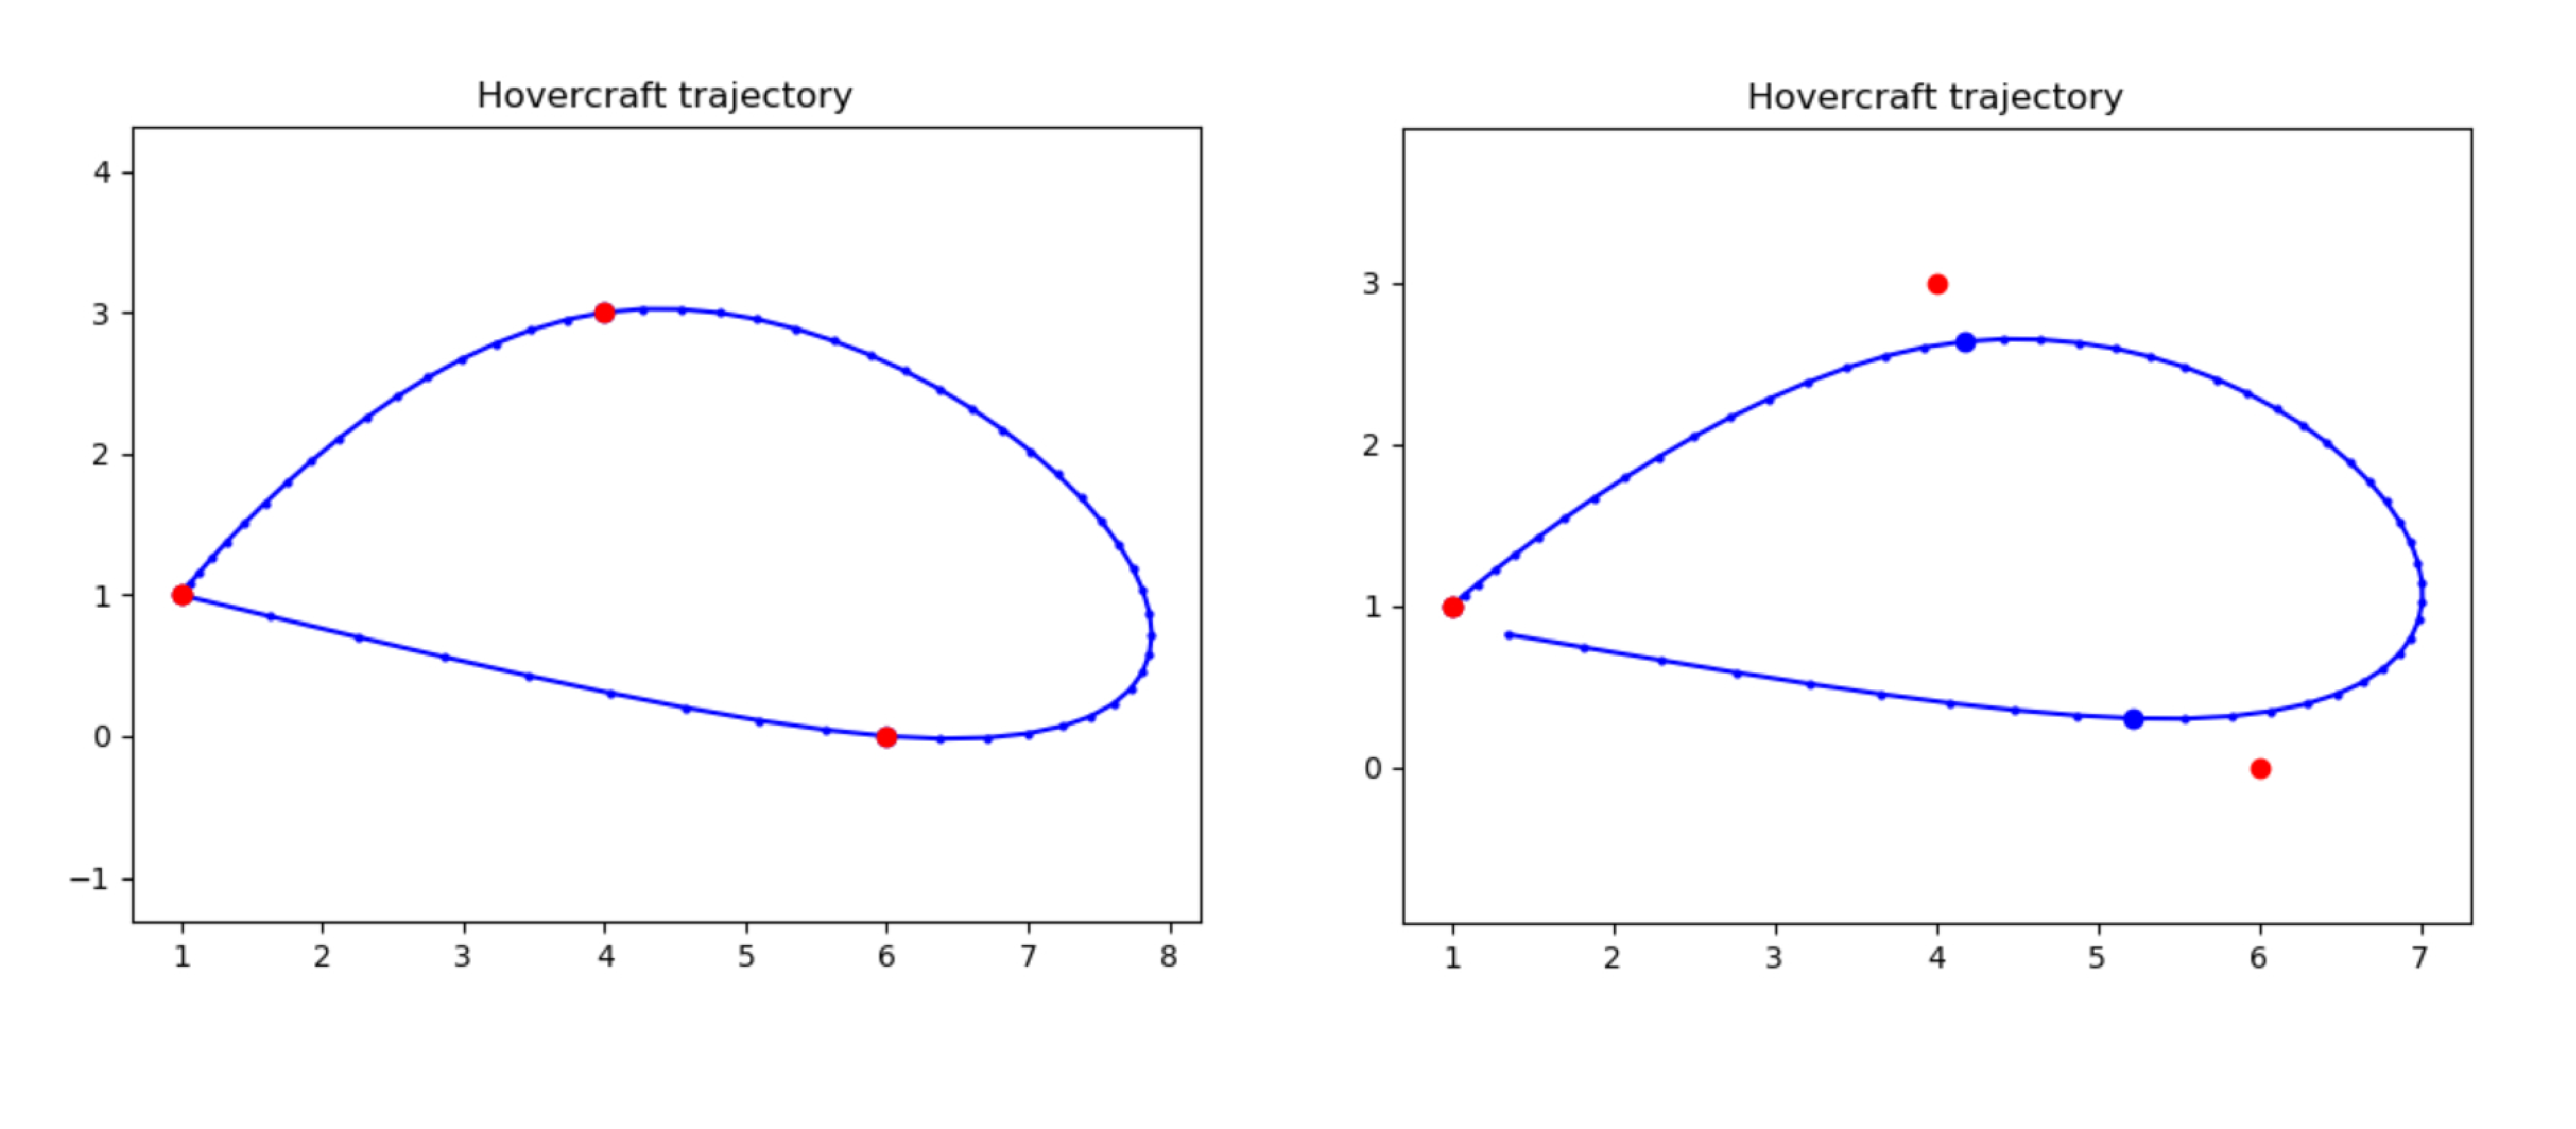
\includegraphics[width=12cm]{aeroglisseur.pdf}
   \end{center}
    \end{figure}
The code is available \href{https://github.com/Cindy-dotcom1/MLA/blob/master/hovercraft_optimization.py}{\textit{\underline{here}}}.
 \end{frame}
 %%%%%%%%%%%%%%%%%%%%%%%%%%%%%%%%%%%%%%%%%%%%%%%%%%%%%
 \begin{frame}{Moving Average reminder}
\begin{block}{Model}
Moving average model is :
$$\forall t \in \{1,....,T\}, \ y_t = w_1 u_t + w_2 u_{t-1} + ... + w_k u_{t-k+1}$$
where :
\begin{itemize}
    \item $(u_t)_{t \in {1...,T}}$ is the time serie of input date ;
    \item $(y_t)_{t \in {1...,T}}$ is the time serie of output date ;
    \item k is the size for which each output is a weighted combination of k previous inputs ;
    \item $(w_i)_{i \in {1...,k}}$ is the weight of each input.
\end{itemize}
\end{block}
 \end{frame}
 %%%%%%%%%%%%%%%%%%%%%%%%%%%%%%%%%%%%%%%%%%%%%%%%%%%
\begin{frame}{Moving Average on the dataset "Données comptages Totem"}
Thanks to this dataframe, we want to modelize the frequency, using of moving average, of passage of cyclists in front of the totem pole located at Place Albert 1er. \\
Our process to do this, is :
\begin{enumerate}
    \item Count the number of cyclists passed per day ;
    \item Modelize the moving average to modelize the frequency of passage of cyclists ;
    \item Calculate error of prediction.
\end{enumerate}
\end{frame}
 %%%%%%%%%%%%%%%%%%%%%%%%%%%%%%%%%%%%%%%%%%%%%%%%%%%
 \begin{frame}{Moving Average on the dataset "Données comptages Totem" - Plot}
\begin{figure}[!h]
     \begin{center}
   \caption{\label{étiquette}Moving average to predict frequency of passage of cyclists (left) and prediction error (right).}
   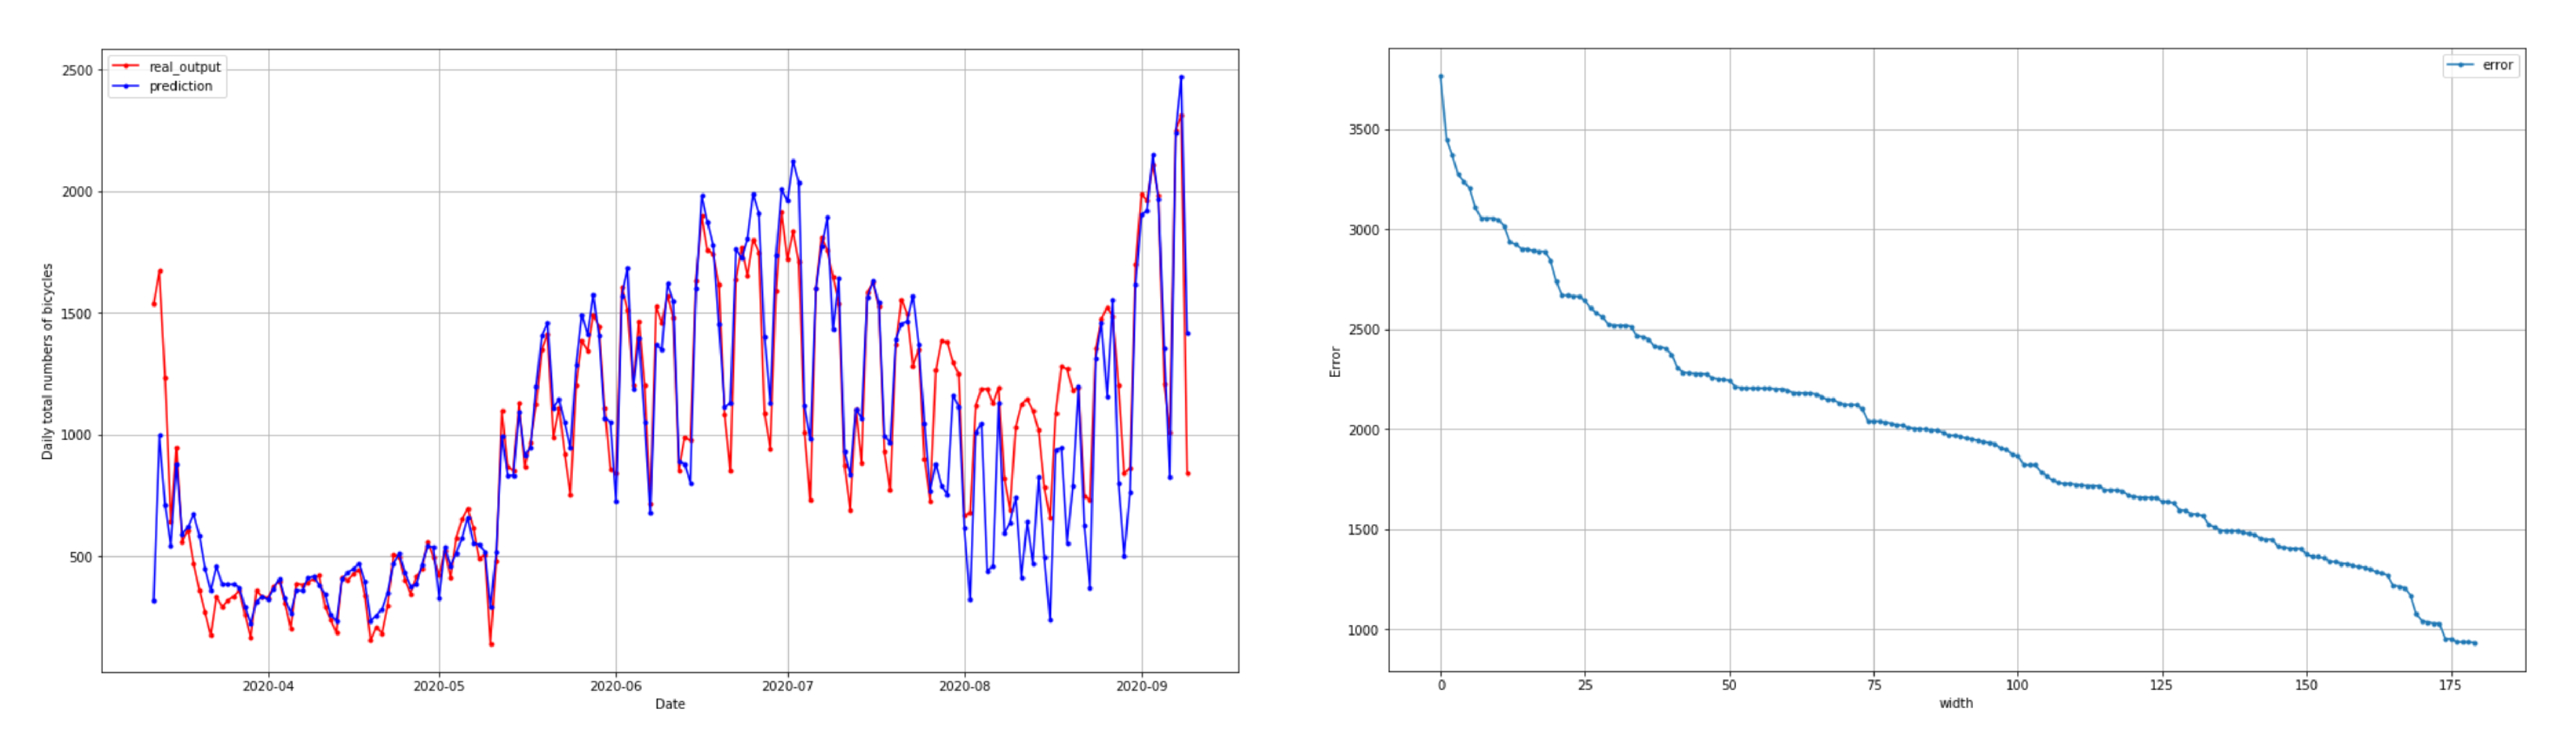
\includegraphics[width=12cm]{prediction_totem.pdf}
   \end{center}
    \end{figure}
The code is available \href{https://github.com/Cindy-dotcom1/MLA/blob/master/Notebooks/Moving_Average_Totem.ipynb}{\textit{\underline{here}}}.
 \end{frame}
  %%%%%%%%%%%%%%%%%%%%%%%%%%%%%%%%%%%%%%%%%%%%%%%%%%%
 \begin{frame}{Moving Average on the dataset "Accidents vélos"}
With the data "Accidents vélos", we want to predict, thanks to moving average calculate over the years 2005 to 2017, the frequency of
bicycle accidents in 2018. \\
Our process to do this is :
\begin{enumerate}
    \item Count the number of cyclists passed per day over the years of 2005 to 2017 (or 2016) ;
    \item Modelize the moving average to predict the frequency of bike accidents in 2018 (or 2017) ;
    \item Calculate error of prediction.
\end{enumerate}
\end{frame}
 %%%%%%%%%%%%%%%%%%%%%%%%%%%%%%%%%%%%%%%%%%%%%%%%%%%
 \begin{frame}{Moving Average on the dataset "Accidents vélos" - Plot}
\begin{figure}[!h]
     \begin{center}
   \caption{\label{étiquette}Moving average to predict frequency of bike accidents by day in 2018 (left) and prediction error (right).}
   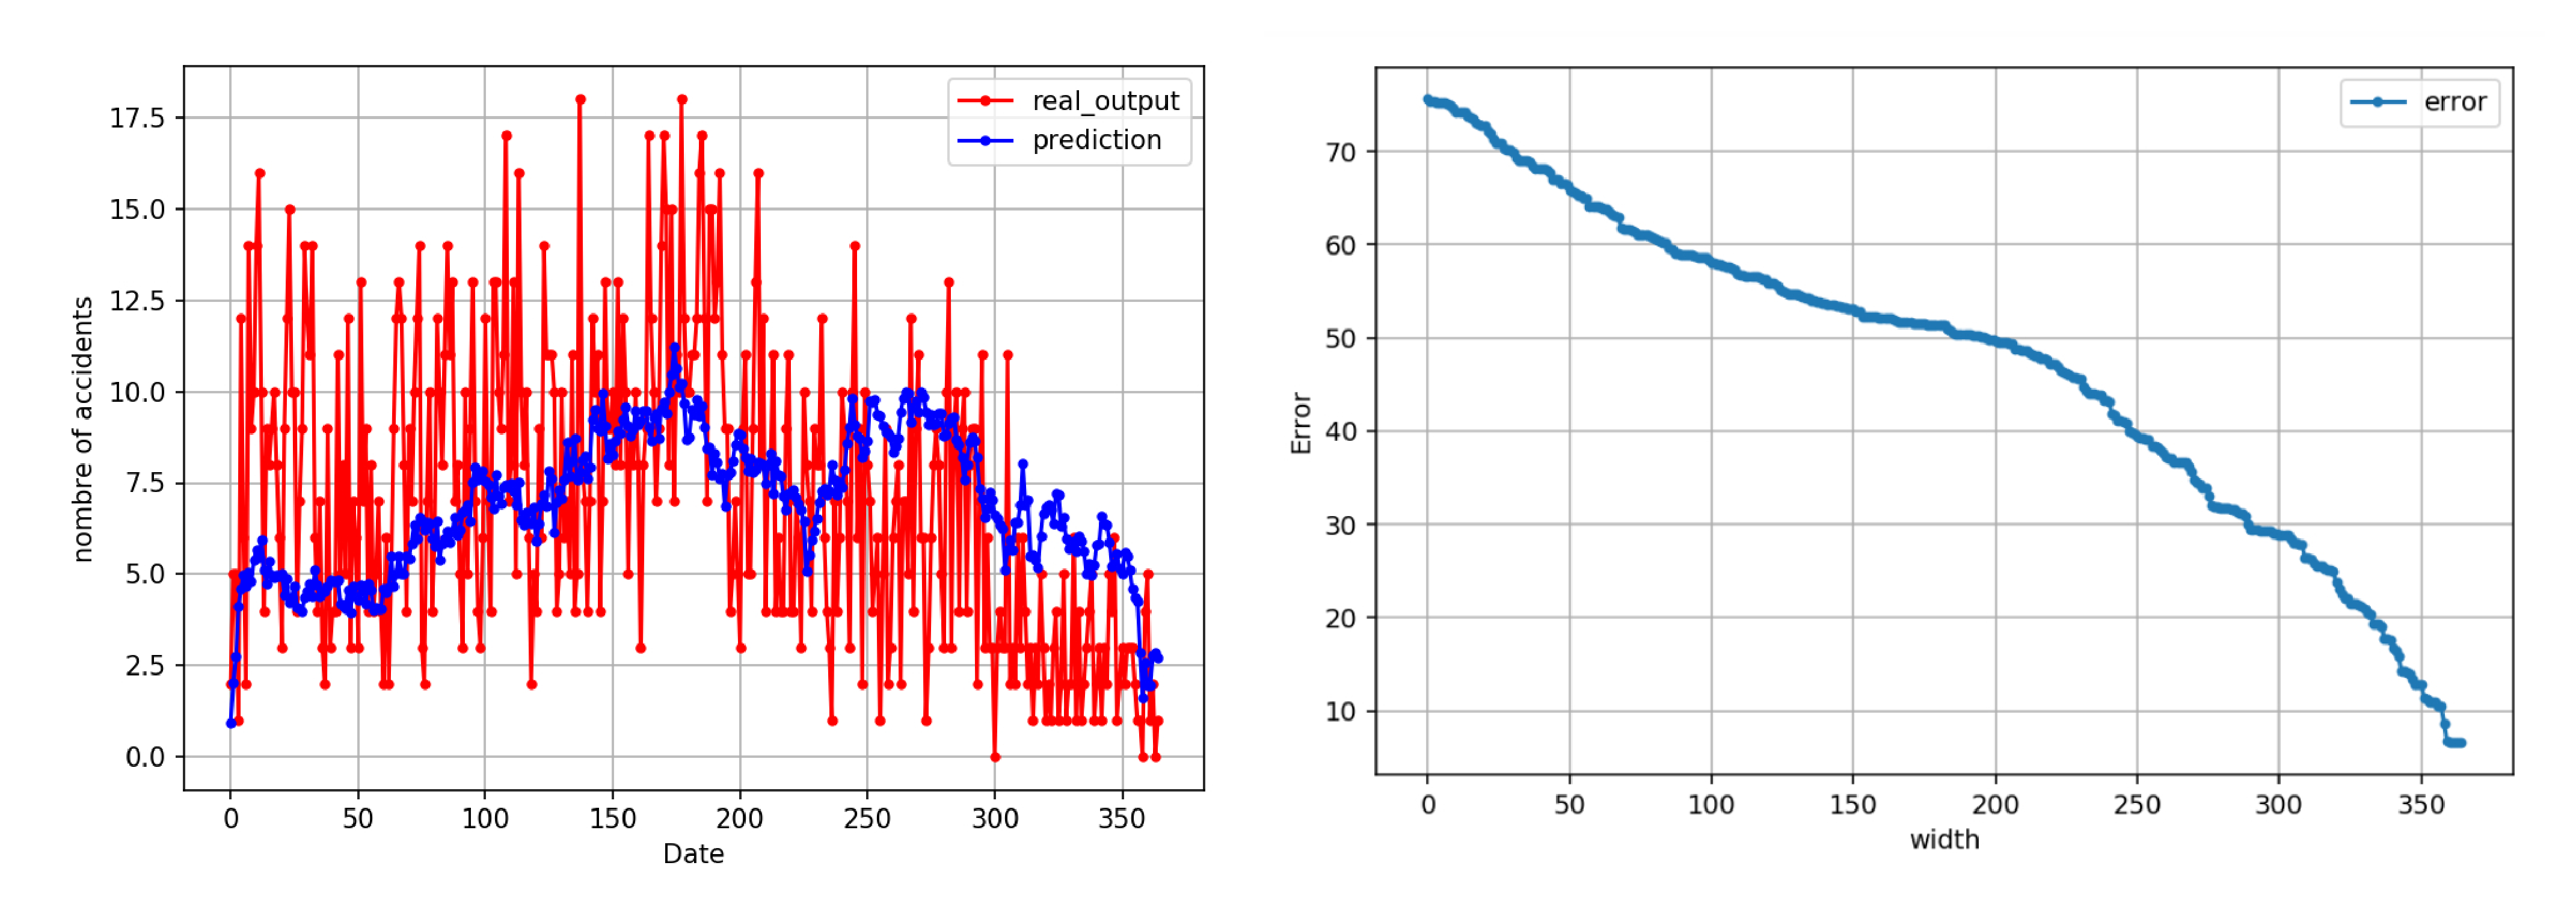
\includegraphics[width=12cm]{prediction_bicycle_db.pdf}
   \end{center}
    \end{figure}
The code is available \href{https://github.com/Cindy-dotcom1/MLA/blob/master/Notebooks/bicycle_daily_accident_prediction.ipynb}{\textit{\underline{here}}}.
 \end{frame}
  %%%%%%%%%%%%%%%%%%%%%%%%%%%%%%%%%%%%%%%%%%%%%%%%%%%
   %%%%%%%%%%%%%%%%%%%%%%%%%%%%%%%%%%%%%%%%%%%%%%%%%%%
 \begin{frame}{Moving Average on the dataset "Accidents vélos" - Plot}
\begin{figure}[!h]
     \begin{center}
   \caption{\label{étiquette}Moving average to predict frequency of bike accidents in 2018 by days of the week (left) and prediction error (right).}
   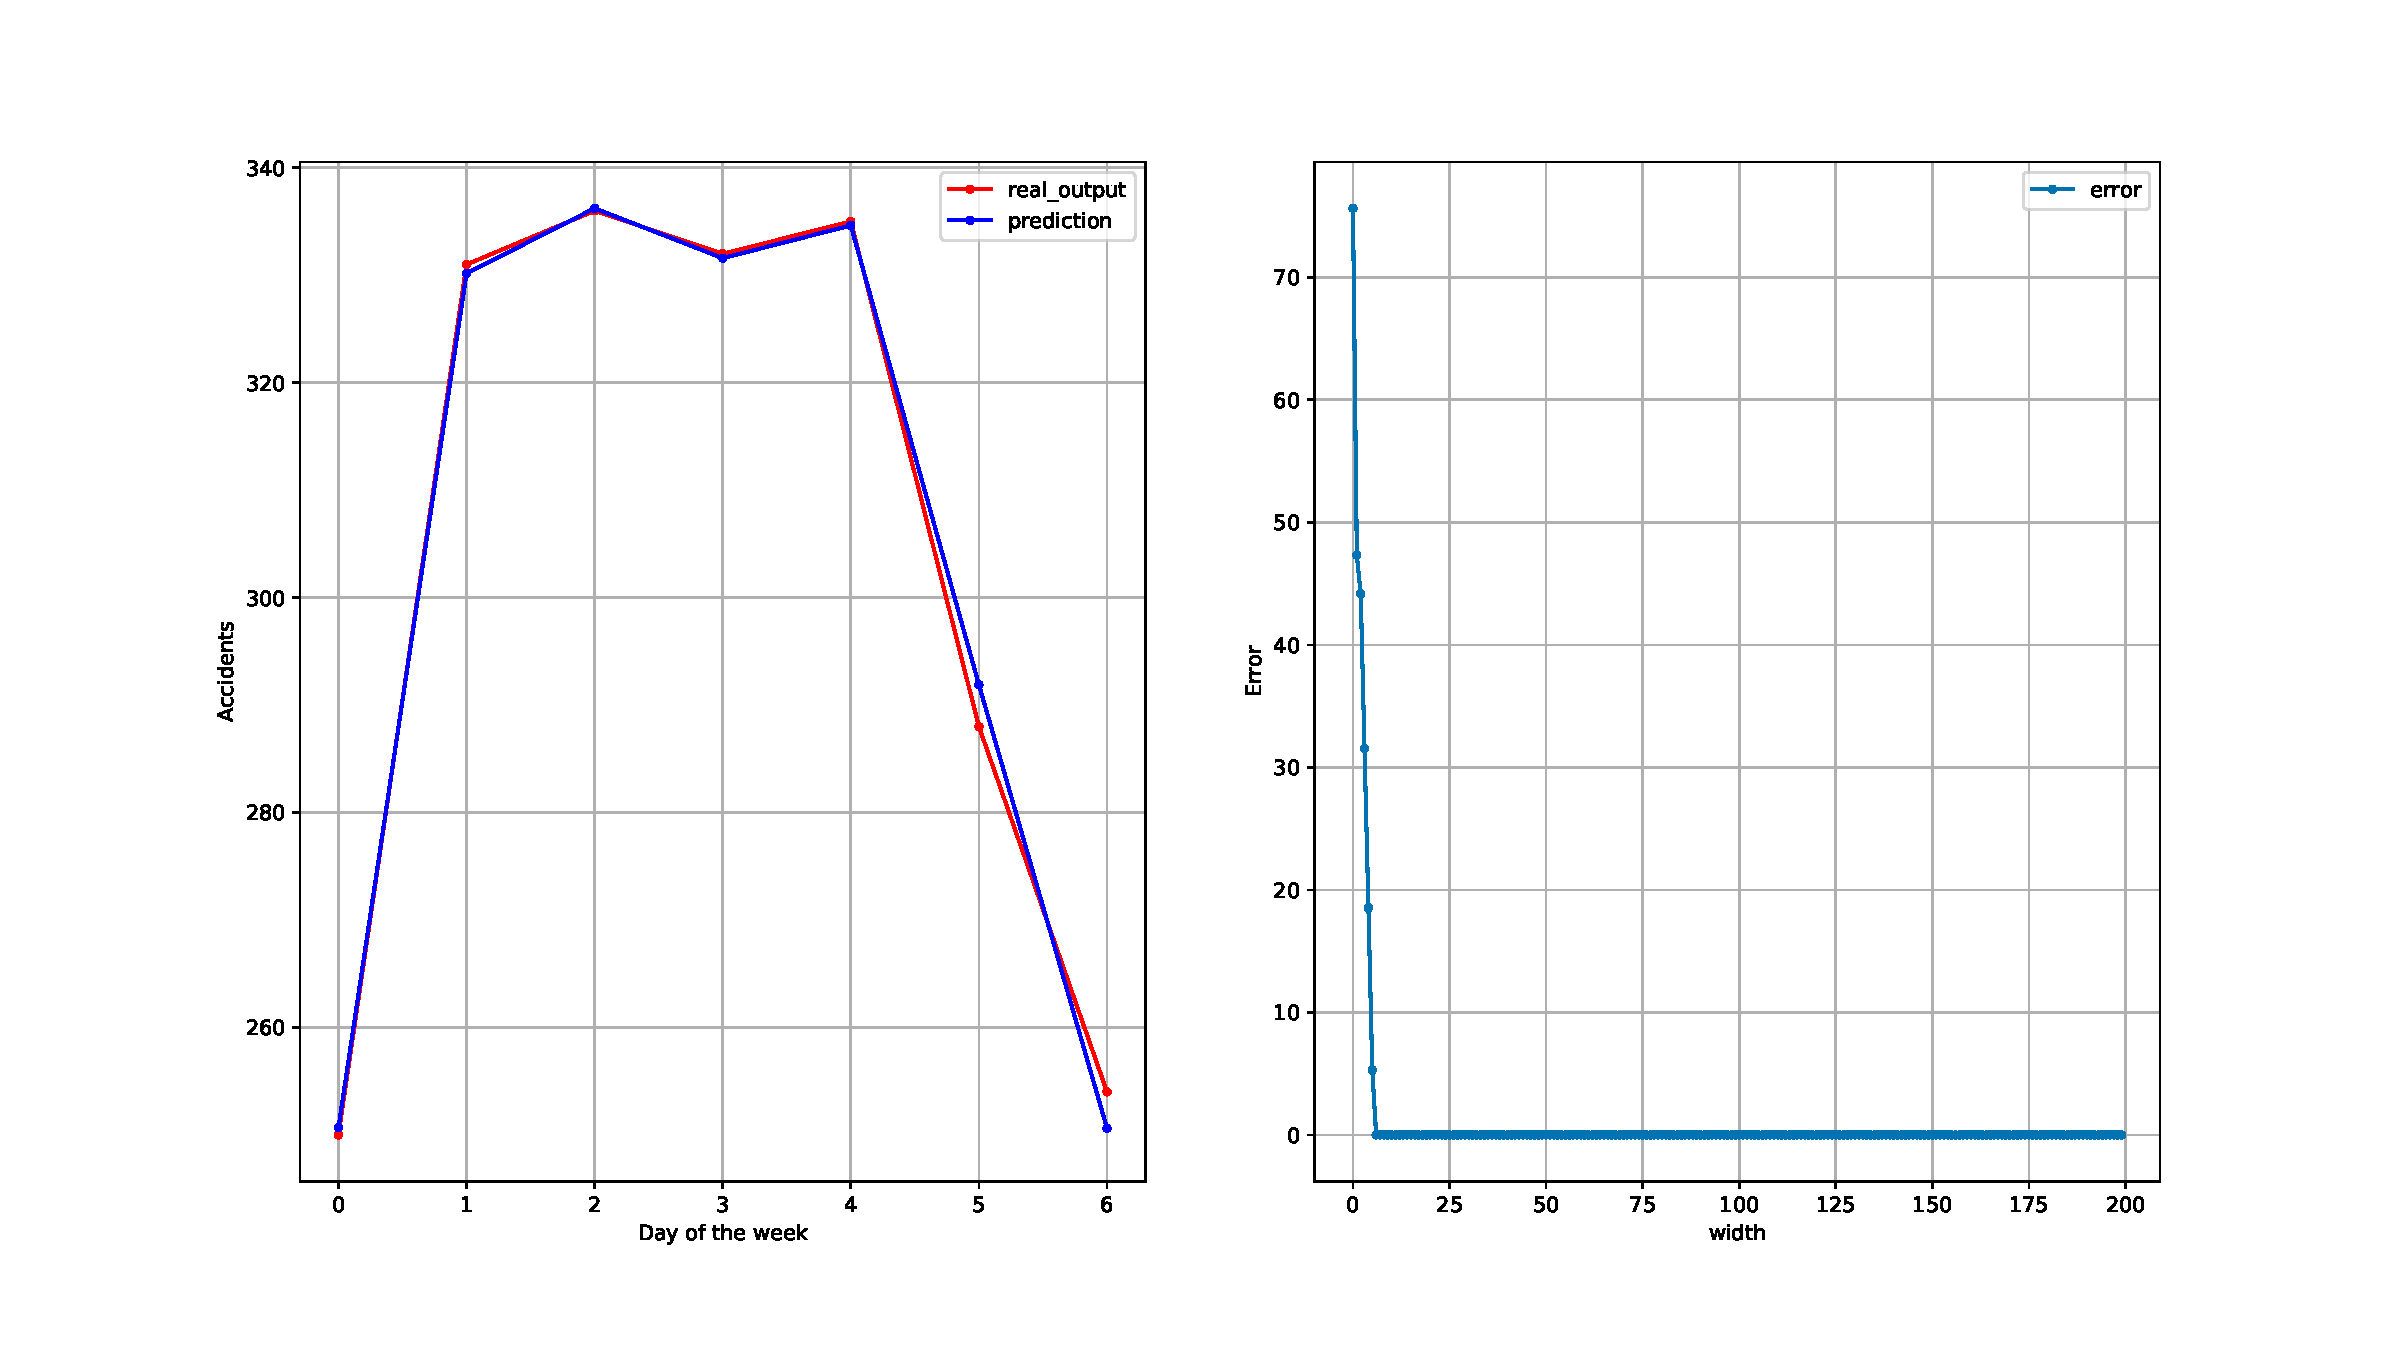
\includegraphics[width=12cm]{2018}
   \end{center}
    \end{figure}
The code is available \href{https://github.com/Cindy-dotcom1/MLA/blob/master/Notebooks/Bicycle_2018.ipynb}{\textit{\underline{here}}}.
 \end{frame}
  %%%%%%%%%%%%%%%%%%%%%%%%%%%%%%%%%%%%%%%%%%%%%%%%%%%
    %%%%%%%%%%%%%%%%%%%%%%%%%%%%%%%%%%%%%%%%%%%%%%%%%%%
 \begin{frame}{Moving Average on the dataset "Accidents vélos" - Plot}
\begin{figure}[!h]
     \begin{center}
   \caption{\label{étiquette}Moving average to predict frequency of bike accidents in 2017 by days of the week (left) and prediction error (right).}
   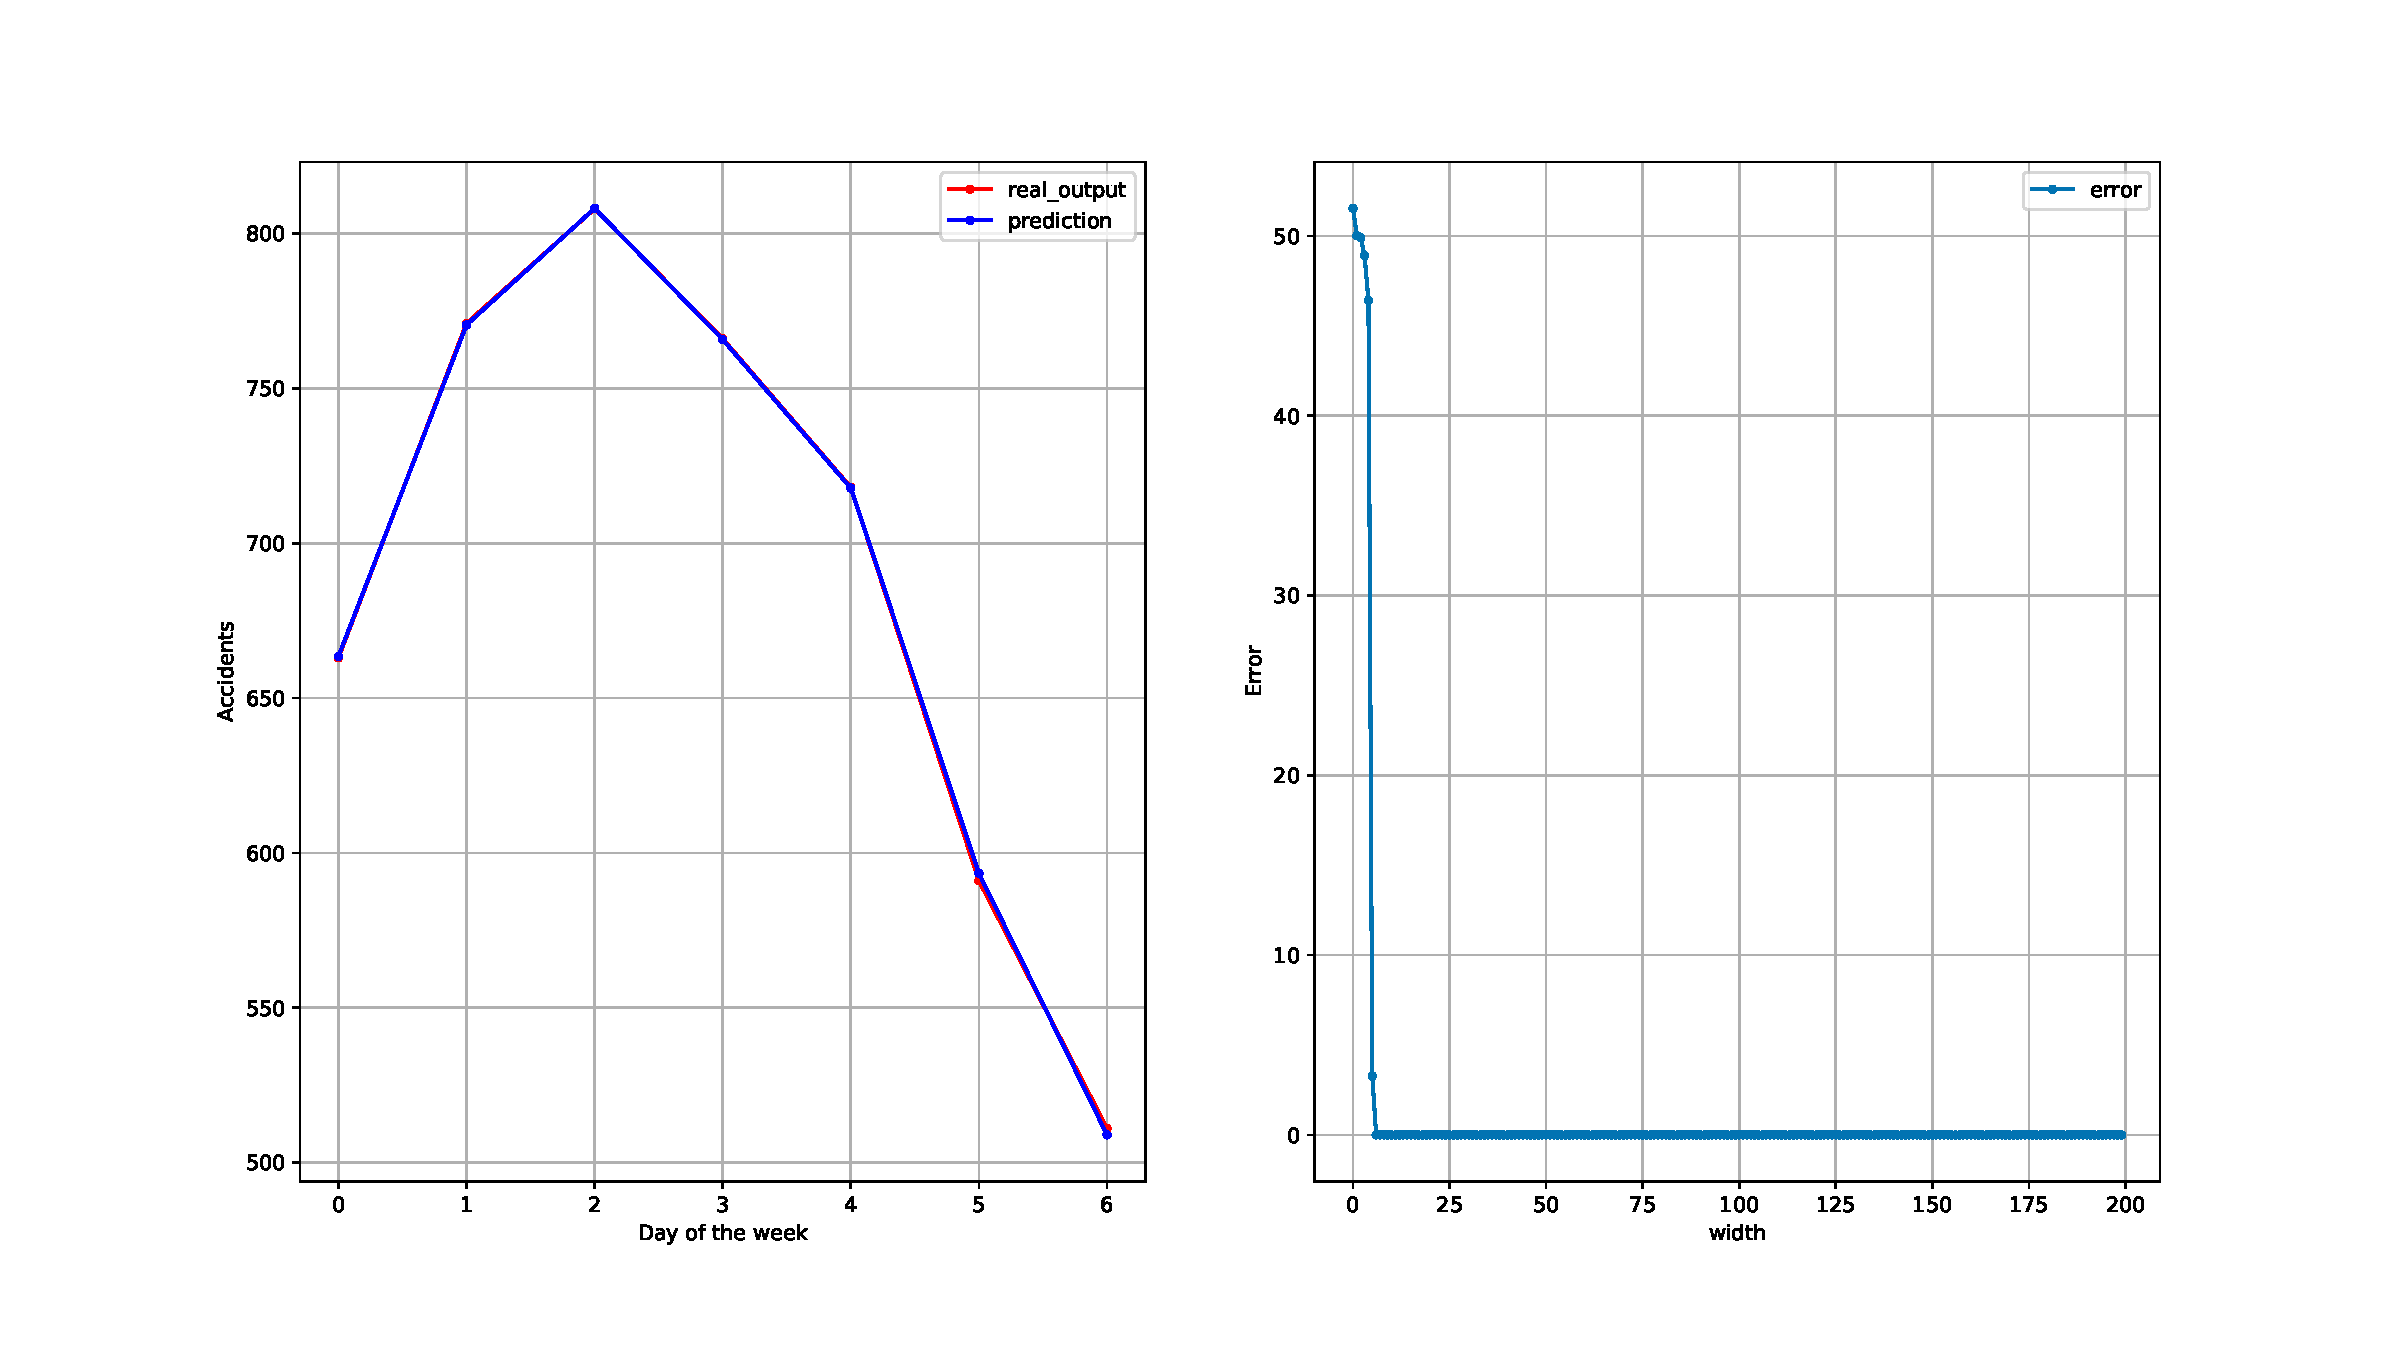
\includegraphics[width=12cm]{2017}
   \end{center}
    \end{figure}
The code is available \href{https://github.com/Cindy-dotcom1/MLA/blob/master/Notebooks/Bicycle-2017.ipynb}{\textit{\underline{here}}}.
 \end{frame}
  %%%%%%%%%%%%%%%%%%%%%%%%%%%%%%%%%%%%%%%%%%%%%%%%%%%
\begin{frame}{Bibliography}
[1] Joseph Salmon, \textit{Modéle linéaire avancé : Optimisation}, 2019, \url{http://josephsalmon.eu/enseignement/Montpellier/HMMA307/Optimisation.pdf} ; \\
[2] Laurent Lessard \textit{Introduction to optimization}, 2017,

\printbibliography
\end{frame}
 %%%%%%%%%%%%%%%%%%%%%%%%%%%%%%%%%%%%%%%%%%%%%%%%%%%%%%%%%%%%%%%%%%%%%%%%%%%%%%



\end{document}